\documentclass[]{article}
\usepackage[english, greek]{babel}
\usepackage[margin=2.5cm]{geometry}
\usepackage{fontspec}
\usepackage{graphicx}
\usepackage{subcaption}
\usepackage{listings}
\usepackage{float}
\usepackage{todonotes}
\usepackage{hyperref}

% Define custom colors
\definecolor{codegreen}{rgb}{0,0.6,0}
\definecolor{codegray}{rgb}{0.5,0.5,0.5}
\definecolor{codepurple}{rgb}{0.58,0,0.82}
\definecolor{backcolour}{rgb}{0.95,0.95,0.92}

% Setup the language and colors
\lstset{
	language=Python,
	backgroundcolor=\color{backcolour},   
	commentstyle=\color{codegreen},
	keywordstyle=\color{magenta},
	numberstyle=\tiny\color{codegray},
	stringstyle=\color{codepurple},
	basicstyle=\ttfamily\footnotesize,
	breakatwhitespace=false,         
	breaklines=true,                 
	keepspaces=true,                 
	numbers=left,                    
	numbersep=5pt,                  
	showspaces=false,                
	showstringspaces=false,
	showtabs=false,                  
	tabsize=2,
}

%opening
\title{\textbf{Όραση Υπολογιστών}\\ 1η Σειρά Εργαστηριακών Ασκήσεων}
\author{Ραφτόπουλος Μιχαήλ - ΑΜ: 03120114}
\date{Εαρινό Εξάμηνο 2024}

\begin{document}
	\setmainfont{Liberation Serif}
	\maketitle
	
	\textit{Σημείωση: Προκειμένου να διατηρηθεί συνοπτική η αναφορά, αφαιρέθηκε ο πηγαίος κώδικας. Εάν θέλετε να δείτε την αναφορά με τον πηγαίο κώδικα, κοιτάξτε το αρχείο 'lab1\_report\_withcode.pdf'.}
	
	\section*{Μέρος 1: Ανίχνευση Ακμών σε Γκρίζες Εικόνες}
	\subsection*{1.1 Δημιουργία Εικόνων Εισόδου}
	\paragraph{1.1.1} Διαβάζουμε την εικόνα εισόδου και την μετατρέπουμε από BGR  σε Grayscale.
	\paragraph{1.1.2} Προκειμένου να βρεθούν οι κατάλληλες τυπικές αποκλίσεις $\sigma_n$ με ακρίβεια ώστε να έχουμε τα ζητούμενα PSNR, αλλά και για ευκολότερη μελλοντική χρήση, υλοποιήθηκε η συνάρτηση PSNRnoise(). Η συνάρτηση αυτή δέχεται μια εικόνα και μια τιμή PSNR και της εφαρμόζει λευκό γκαουσιανό θόρυβο, με την κατάλληλη τυπική απόκλιση $\sigma_n$. Για τον υπολογισμό αυτό χρησιμοποιείται ένας απλός αλγόριθμος δυαδικής αναζήτησης.
	Εφαρμόζουμε τον θόρυβο στην εικόνα και παρουσιάζουμε τα αποτελέσματα\\
	\begin{figure}[H]
		\centering
		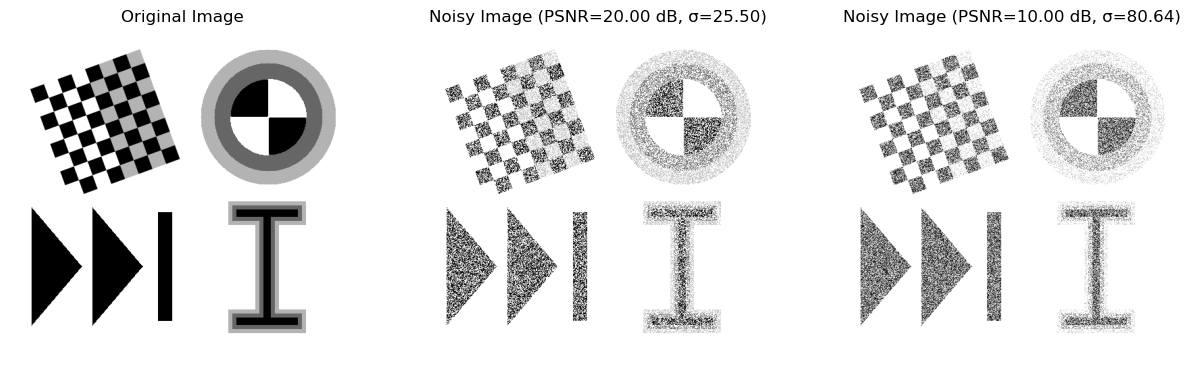
\includegraphics[width=\linewidth]{output1}
		\caption{Η αρχική εικόνα, εικόνα με γκαουσιανό θόρυβο PSNR=20dB, εικόνα με γκαουσιανό θόρυβο PSNR=10dB}
	\end{figure}
	\newpage
	
	\subsection*{1.2 Υλοποίηση Αλγορίθμων Ανίχνευσης Ακμών}
	\paragraph{1.2.1} Υλοποιήθηκαν οι δύο συναρτήσεις που επιστρέφουν τις ζητούμενες αποκρίσεις. Και οι δύο συναρτήσεις χρησιμοποιούν αυθαίρετα $\sigma = 5$. Το βέλτιστο $\sigma$ θα βρεθεί αργότερα στην εργασία.
	\paragraph{1.2.2} Εφαρμόζουμε τα ζητούμενα φίλτρα $L_1$ και $L_2$ και εμφανίζουμε τα αποτελέσματα. Στην προκειμένη περίπτωση χρησιμοποιείται η θορυβοποιημένη εικόνα με PSNR=20dB.
	\begin{figure}[H]
		\centering
		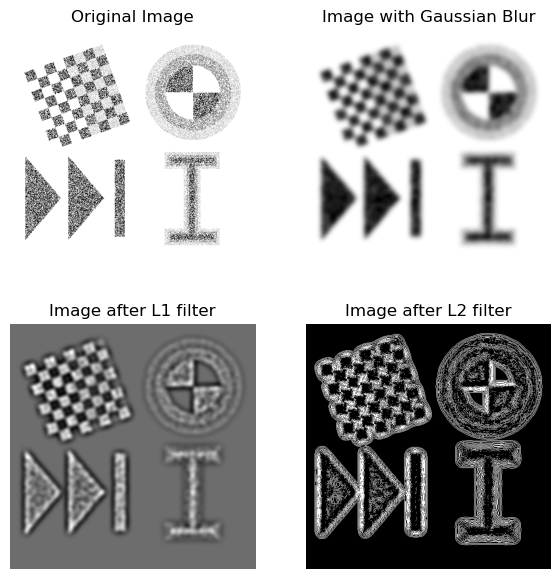
\includegraphics[width=\linewidth/2]{output2}
		\caption{Η αρχική εικόνα, μετά από το φίλτρο G, μετά το φίλτρο LoG, μετά τα μορφολογικά φίλτρα}
	\end{figure}
	\paragraph{1.2.3} Γίνεται η προσέγγιση των zero-crossings. Χρησιμοποιείται ο προτεινόμενος αλγόριθμος, δημιουργείται δηλαδή η δυαδική εικόνα και εντοπίζεται το περίγραμμα με χρήση των κατάλληλων μορφολογικών τελεστών. Εμφανίζονται τα αποτελέσματα
	\begin{figure}[H]
		\centering
		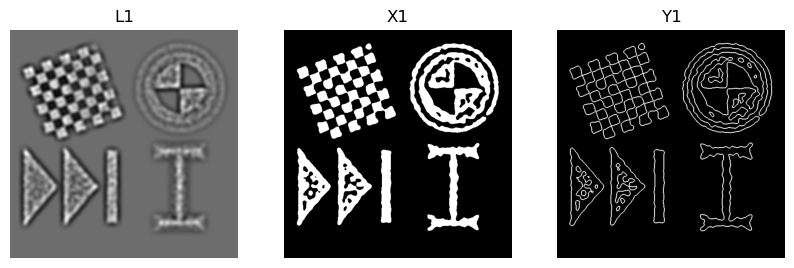
\includegraphics[width=\linewidth]{output3}
		\caption{\\L1: Η εικόνα μετά το φίλτρο LoG\\X1: Η δυαδική εικόμα της L1\\Y1: Το περίγραμμα της X1}
	\end{figure}
	\paragraph{1.2.4} Απορρίπτονται οι ακμές σε ομαλές περιοχές. Θεωρούμε αυθαίρετα $\theta_{edge}=0.1$. Το βέλτιστο $\theta_{edge}$ θα βρεθεί αργότερα στην εργασία. Εμφανίζονται τα αποτελέσματα.
	\begin{figure}[H]
		\centering
		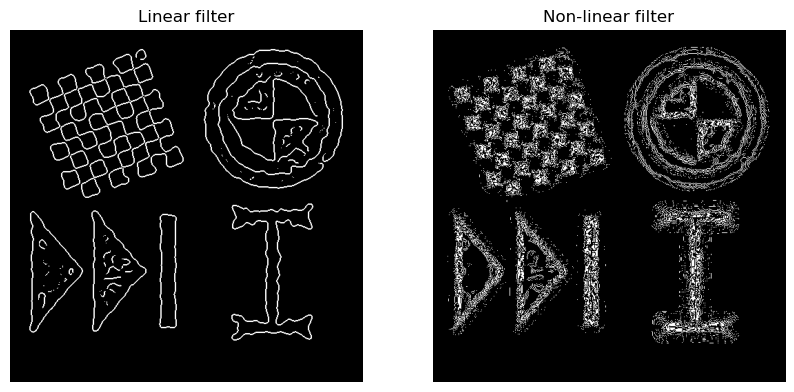
\includegraphics[width=\linewidth]{output4}
		\caption{\\Αριστερά: Το τελικό περίγραμμα της εικόνας με χρήση γραμμικού φίλτρου\\Δεξιά: Το τελκό περίγραμμα της εικόνας με χρήση μη γραμμικού μορφολογιού φίλτρου}
	\end{figure}
	\paragraph{} Τέλος, συνθέτουμε τα παραπάνω βήματα στη ζητούμενη συνάρτηση EdgeDetect()
	\subsection*{1.3 Αξιολόγηση Αποτελεσμάτων Ανίχνευσης Ακμών}	
	\paragraph{1.3.1} Εφαρμόζουμε στην εικόνα τους κατάλληλους μορφολογικούς τελεστές και κατωφλιοποιούμε το αποτέλεσμα, κατασκευάζουμε την εικόνα Τ, με τις πραγματικές ακμές. Θεωρόντας $theta_realedge\=1$, παίρνουμε το προσδοκώμενο αποτέλεσμα.
	\begin{figure}[H]
		\centering
		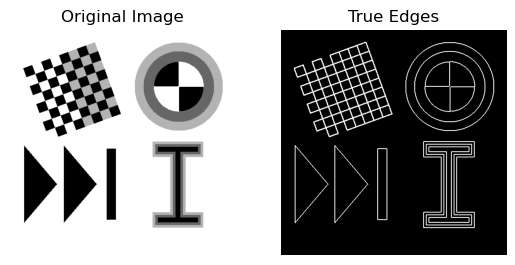
\includegraphics[width=\linewidth]{output5}
		\caption{Η αρχική εικόνα και οι ακμές της}
	\end{figure}	
	\paragraph{1.3.2} Ορίζεται η συνάρτηση score(), που δέχεταιμια εικόνα με τις εκτιμόμενες ακμές και την εικόνα με τις πραγματικές ακμές και υπολογίζει την παράμετρο C, σύμφωνα με τον δωσμένο τύπο.
	\paragraph{1.3.3} Εφαρμόζουμε την συνάρτηση EdgeDetect() στην εικόνα με PSNR=20dB και PSNR=10dB αντίστοιχα, δοκιμάζοντας χειροκίνητα διαφορετικές παραμέτρους, με μέθοδο όμοια του αλγορίθμου Gradient Descent. Οι τιμές που οδήγησαν στα (τοπικά) βέλτιστα score φαίνονται στην εικόνα παρακάτω.
		\begin{figure}[H]
		\centering
		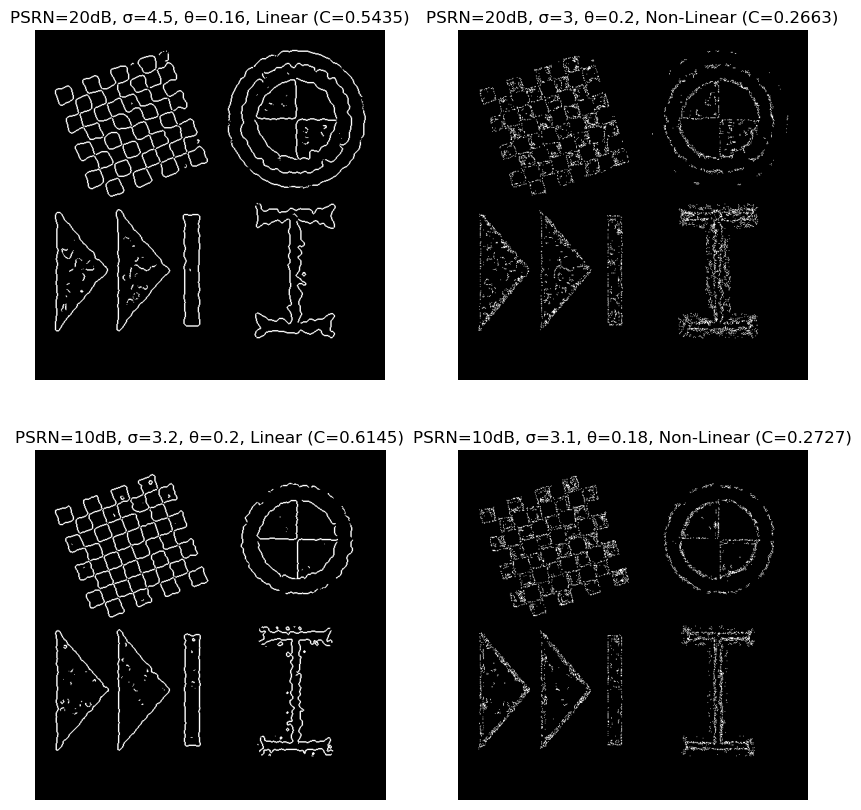
\includegraphics[width=0.8\linewidth]{output6}
		\caption{Τα τελικά αποτελέσματα των δύο αλγορίθμων (L1\&L2), μετά από δοκιμές πολλών τιμών παραμέτρων}
	\end{figure}
	\paragraph{Παρατηρήσεις: }
	\begin{itemize}
		\item Οι "βέλτιστες" αυτές τιμές βρέθηκαν προσεγγιστικά χρησιμοποιώντας χειροκίνητη μέθοδο. Για να βρεθούν οι πραγματικά βέλτιστες παράμετροι θα πρέπει να εφαρμοστεί επαναληπτικά ο αλγόριθμος Gradient Descent, από διαφορετικά σημεία εκκίνησης κάθε φορά, για να αποφευχθούν τυχόν τοπικά βέλτιστες λύσεις.
		\item Ο αλγόριθμος που αξιοποιεί το γραμμικό φίλτρο LoG έχει οδηγεί σε σημαντικά καλύτερα αποτελέσματα (τουλάχιστον με το εύρος παραμέτρων που δοκιμάστηκαν)
		\item Το γραμμικό φίλτρο LoG φαίνεται να προσεγγίζει τις ακμές με συνεχείς γραμμές. Αντιθέτως, το μορφολογικό φίλτρο φαίνεται να κατασκευάζει τις ακμές με ανεξάρτητα μεταξύ τους σημεία.
		\item Επαναλαμβάνοντας το πρόγραμμα με ακριβώς τις ίδιες παραμέτρους οδηγούμαστε κάθε φορά σε ελαφρώς διαφορετικά αποτελέσματα. Θεωρώ ότι αυτό οφείλεται στο στάδιο της θορυβοποίησης που περιλαμβάνει, έστω σε μικρή κλίμακα, τον παράγοντα της "τύχης".
	\end{itemize}
	\subsection*{1.4 Εφαρμογή των Αλγορίθμων Ανίχνευσης Ακμών σε Πραγματικές Εικόνες}	
	\paragraph{1.4.1} Φορτώνουμε την εικόνα 'butterfly.jpg' και εφαρμόζουμε τη συνάρτηση EdgeDetect().
	\paragraph{1.4.2} Δοκιμάζουμε όπως προηγουμένως διαφορετικές τιμές για τις παραμέτρους του αλγορίθμου. Οι βέλτιστες που βρεθήκαν φαίνονται στην εικόνα\\
	\begin{figure}[H]
		\centering
		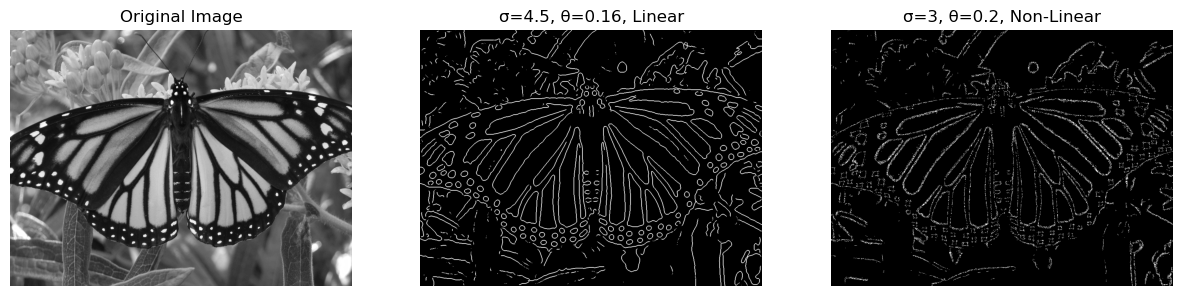
\includegraphics[width=\linewidth]{output7}
		\caption{Τα τελικά αποτελέσματα των δύο αλγορίθμων (L1\&L2), μετά από δοκιμές πολλών τιμών παραμέτρων}
	\end{figure}
	\paragraph{Παρατηρήσεις:}
	\begin{itemize}
		\item Όταν έχουμε μικρό $\sigma_n$,  τόσο περισσότερες λεπτομέρειες περιλαμβάνονται στις ακμές. στην περίπτωση της πραγματικής εικόνας, το αποτέλεσμα είναι αρκετά ικανοποιητικό,. Αν προσθέσουμε όμως θόρυβο, τότε αυτός λαμβάνεται ως ακμή, πράγμα ανεπιθύμιτο.
		\item Όσο αυξάνουμε το $\sigma_n$,  συμπεριλαμβάνονται όλο και λιγότερες λεπτομέρειες και οι ακμές που βρίσκουμε ομαλοποιούνται.
		\item Όμοια με το $\sigma_n$, έτσι και το $\theta_{edge}$ όταν είναι πολύ μικρό συμπεριλαμβάνονται πολλές "λεπτομέρεις". Εδώ όμως οι "λεπτομέρειες" είναι απλά περιοχές με ελαφρώς απότομη μεταβολή στην φωτεινότητα και που δε θα θεωρούσαμε ακμές. Το τελικό αποτέλεσμα είναι περιοχές με ένα "θορυβόδες" πλήθος ακμών. Σε κάθε περίπτωση λοιπόν το υπερβολικά μικρό $\theta_{edge}$ είναι ανεπιθύμητο.
		\item Καθώς μεγαλώνουμε το $\theta_{edge}$, ο αριθμός αυτών των περιοχών με ασήμαντη μεταβολή στη φωτεινότητα μειώνεται, φτάνοντας ένα βέλτιστο σημειο. Αν συνεχίσουμε να αυξάνουμε περαιτέρω, θα αρχίσουν να περιορίζονται ακόμα και οι επιθυμητές ακμές, μέχρι να φτάσουμε σε μια τελείως σκοτεινή εικόνα.
	\end{itemize}
	\begin{figure}[H]
		\centering
		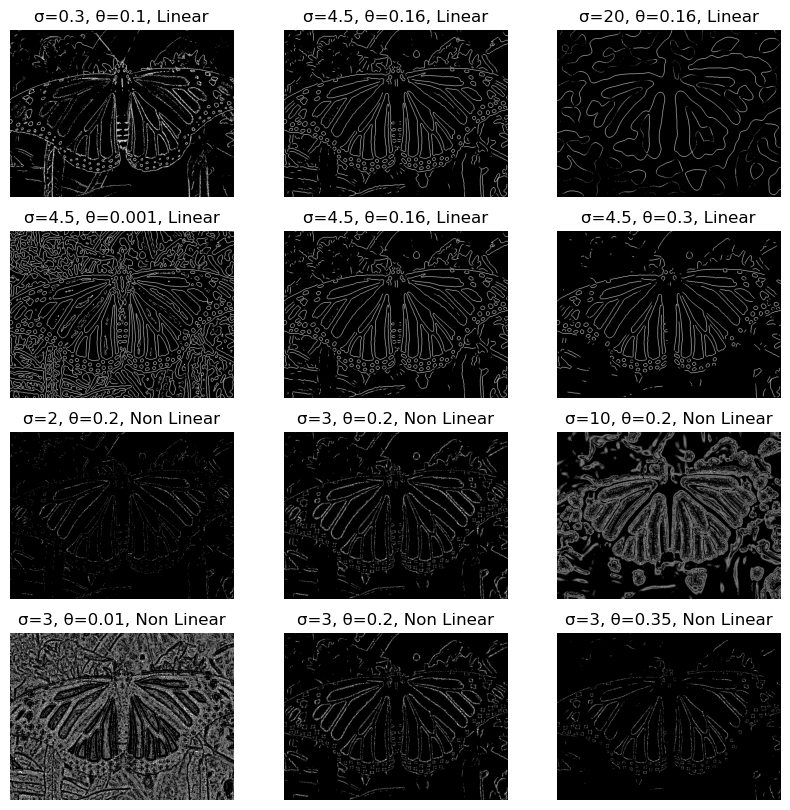
\includegraphics[width=\linewidth]{output8}
		\caption{Η εικόνα butterfly.jpg, μετά από δοκιμές διαφόρων παραμέτρων}
	\end{figure}
	
	\newpage
	\section*{Μέρος 2: Ανίχνευση Σημείων Ενδιαφέροντος}
	\subsection*{2.1 Ανίχνευση γωνιών}
	\paragraph{2.1.1} Υπολογίζονται τα στοιχεία του δομικού τελεστή $J$.

	\paragraph{2.1.2} Υπολογίζουμε τις ιδιοτιμές $\lambda_{+}$, $\lambda_{-}$, βγάζοντας αναμενόμενα αποτελέσματα
	\begin{figure}[H]
		\centering
		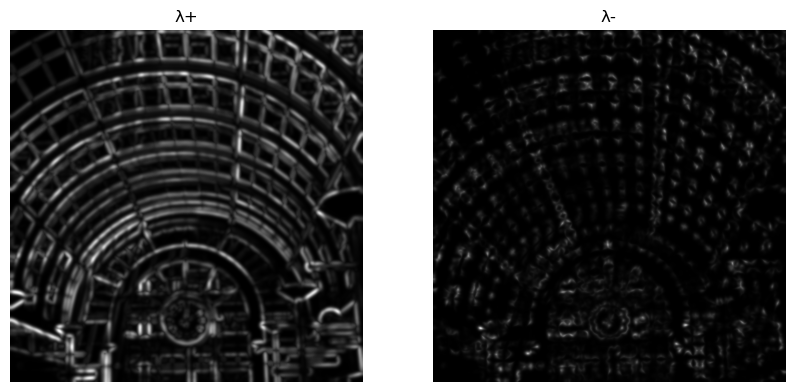
\includegraphics[width=\linewidth]{lambda}
		\caption{λ+ και λ-}
	\end{figure}
	
	\paragraph{2.1.3} Υπολογίζουμε το κριτήριο γωνιότητας και εφαρμόζουμε τις δύο συνθήκες. Τέλος, εμφανίζουμε την εικόνα με πράσινες τελείες στα σημεία που απέμειναν.
		\begin{figure}[H]
		\centering
		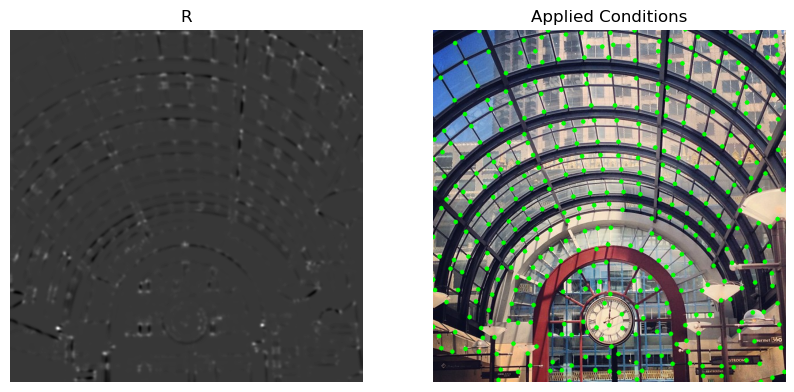
\includegraphics[width=\linewidth]{edges}
		\caption{Μονοκλιμακωτή εύρεση γωνιών}
	\end{figure}
	
	\subsection*{2.2 Πολυκλιμακωτή Ανίχνευση γωνιών}
	\paragraph{2.2.1} Αφού υλοποιήσουμε μια συνάρτηση που περιλαμβάνει τον αλγόριθμο του μέρους 2.1, τρέχουμε τον αλγόριθμο για πολλές κλίμακες.
	\paragraph{2.2.2} Υπολογίζουμε την κανονικοποιημένη LoG για καθεμία από τις κλίμακες. Για κάθε σημείο (x,y) που έχουμε βρει, ελέγχουμε αν $LoG(x,y,\sigma_i)>LoG(x,y,\sigma_{i+1})$ και $LoG(x,y,\sigma_i)>LoG(x,y,\sigma_{i-1})$. Αν δεν ισχύει η συνθήκη, το απορρίπτουμε. Τέλος, οπτικοποιούμε το αποτέλεσμα χρησιμοποιώντας τη συνάρτηση $interest\_points\_visualization()$.
	\begin{figure}[H]
		\centering
		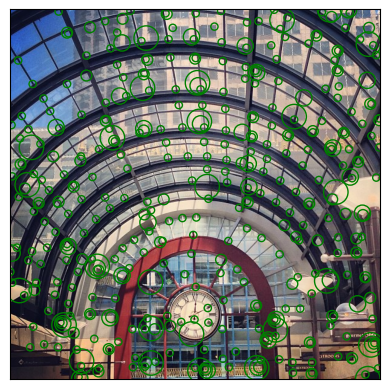
\includegraphics[width=\linewidth/2]{output9}
		\caption{Πολυκλιμακωτό corner detection}
	\end{figure}
	
	\subsection*{2.3 Ανίχνευση Blobs}
	\paragraph{2.3.1} Υπολογίζονται οι μερικές παράγωγοι και το κριτήριο R
	\paragraph{2.3.2}Χρησιμοποιώντας τις ίδιες συνθήκες με το μέρος 2.1, καταλήγουμε σε ορισμένα blobs, τα οποία σημαδεύουμε με πράσινες τελείες.
	
	\begin{figure}[H]
		\centering
		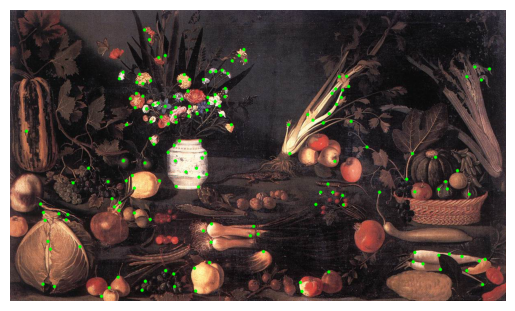
\includegraphics[width=\linewidth/2]{blobs}
		\caption{Μονοκλιμακωτό blob detection}
	\end{figure}
	
	\subsection*{2.4 Πολυκλιμακωτή Aνίχνευση Blobs} 
	\paragraph{2.4.1} Όπως και προηγουμένως, υλοποιούμε τη συνάρτηση $BlobDetect()$. Ακολουθώντας όμοια διαδικασία, υλοποιούμε το normalized $LoG$ και κρατάμε μόνο τα σημεία που είναι μέγιστα σε σχέση με τις γειτονικές τους κλίμακες. Οπτικοποιούμε το αποτέλεσμα.
	\begin{figure}[H]
		\centering
		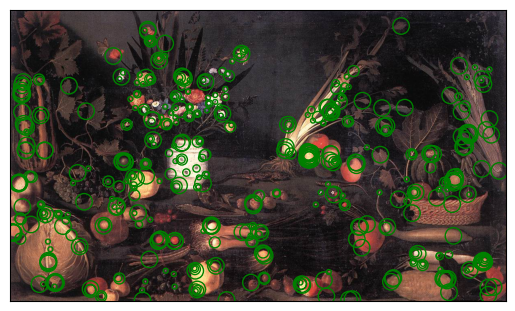
\includegraphics[width=\linewidth/2]{output10}
		\caption{Πολυκλιμακωτό blob detection}
	\end{figure}
	
	\subsection*{2.5 Επιτάχυνση με την χρήση Box Filters και Ολοκληρωτικών Εικόνων (Integral Images)}
	\paragraph{2.5.1} Χρησιμοποιώντας τη συνάρτηση $np.cumsum()$ κατά τους άξονες x και y της αρχικής εικόνας (σε grayscale), υπολογίζουμε την αντίστοιχη πολυκλιμακωτή εικόνα.
	\begin{figure}[H]
		\centering
		
\includegraphics[width=0.5\linewidth]{integral_image}
		\caption{Η ολοκληρωτική εικόνα της εικόνας εισόδου}
	\end{figure}
	
	\paragraph{2.5.2} Υλοποιούμε τη βοηθητική συνάρτηση $int_sum()$, που δέχεται σαν ορίσματα τις διαστάσεις ενός παραθύρου, μια ολοκληρωτική εικόνα και αρχικές συντεταγμένες (x,y) και υπολογίζει το άθροισμα των σημείων της αρχικής εικόνας στο δοσμένο παράθυρο, χρησιμοποιώντας τον τύπο (18) της εκφώνησης. Ύστερα, προκειμένου να υπολογίσουμε τα $D_{xx}$, $D_{yy}$, και $D_{xy}$, διατρέχουμε κάθε σημείο της εικόνας και καλούμε τη συνάρτηση $int_sum()$ (με αρχικό το διατρεχόμενο σημείο), υπολογίζοντας τα αθροίσματα των κατάλληλων περιοχών, ανάλογα με τη συνάρτηση που προσεγγίζουμε. Για το κάθε σημείο, προσθέτουμε ή αφαιρούμε τις περιοχές κατάλληλα, σύμφωνα με τους πυρήνες του σχήματος 2 της εκφώνησης.
	\paragraph{2.5.3} Υπολογίζουμε το αντίστοιχο κριτήριο blob.
\	\paragraph{2.5.4} Για άλλη μια φορά, συνδιάζουμε τα προηγούμενα βήματα σε μια συνάρτηση ($FastBlobDetect()$), η οποία είναι ίδια με την $BlobDetect()$, μόνο που αντί για $L_{xy}$ χρησιμοποιεί τις προσεγγίσεις $D_{xy}$, καθώς και χρησιμοποιεί το αντίστοιχο προσσεγιστικό $R$. Χρησιμοποιούμε τη συνάρτηση και εφαρμόζουμε ακριβώς την ίδια διαδικασία με το μέρος 2.4.1.
	\begin{figure}[H]
		\centering
		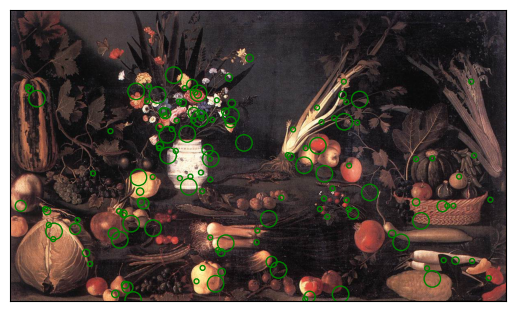
\includegraphics[width=\linewidth]{output11}
		\caption{Πολυκλιμακωτό blob detection με χρήση box filters}
	\end{figure}
	
	\newpage
	
	\section*{Μέρος 3: Εφαρμογές σε Ταίριασμα και Κατηγοριοποίηση Εικόνων με Χρήση Τοπικών Περιγραφητών στα Σημεία Ενδιαφέροντος}
	\subsection*{3.1. Ταίριασμα Εικόνων υπό Περιστροφή και Αλλαγή Κλίμακας}
	\paragraph{3.1.1} Αρχικά, οι αλγόριθμοι που αναπτύχθηκαν στα προηγούμενα μέρη οργανώνονται σε μια σειρά από συναρτήσεις και τροποποιούνται ελαφρώς ώστε τα αποτελέσματα να είναι συμβατά με τις συναρτήσεις του cv24\_lab1\_part3\_utils. Ύστερα, χρησιμοποιούμε τη συνάρτηση matching\_evaluation() με inputs τον Harris Detector και τον περιγραφιτή SURF.
	\begin{lstlisting}[language=, caption={Αποτελέσματα matching\_evaluation() για Harris Detector και περιγραφητή SURF}]
		Avg. Scale Error for Image 1: 0.002
		Avg. Theta Error for Image 1: 0.109
	\end{lstlisting}
	
	\paragraph{3.1.2} Καλούμε τη συνάρτηση matching\_evaluation() για τις διάφορες εισόδους. Παρατηρούμε ότι την καλύτερη επίδοση παρουσιάζουν οι ανιχνευτές Harris και Hessian, με τον περιγραφητή SURF.
	
	\begin{lstlisting}[language=, caption={Αποτελέσματα matching\_evaluation() για διάφορες εισόδους}]
		1. MONOSCALED HARRIS - SURF DESCRIPTOR
		Avg. Scale Error for Image 1: 0.003
		Avg. Theta Error for Image 1: 1.967
		
		2. MONOSCALED HARRIS - HOG DESCRIPTOR
		Avg. Scale Error for Image 1: 0.186
		Avg. Theta Error for Image 1: 22.619
		
		3. MULTISCALED HARRIS - SURF DESCRIPTOR
		Avg. Scale Error for Image 1: 0.002
		Avg. Theta Error for Image 1: 0.109
		
		4. MULTISCALED HARRIS - HOG DESCRIPTOR
		Avg. Scale Error for Image 1: 0.097
		Avg. Theta Error for Image 1: 13.003
		
		5. MONOSCALED HESSIAN - SURF DESCRIPTOR
		Avg. Scale Error for Image 1: 0.027
		Avg. Theta Error for Image 1: 7.759
		
		6. MONOSCALED HESSIAN - HOG DESCRIPTOR
		Avg. Scale Error for Image 1: 0.186
		Avg. Theta Error for Image 1: 7.200
		
		7. MULTISCALED HESSIAN - SURF DESCRIPTOR
		Avg. Scale Error for Image 1: 0.001
		Avg. Theta Error for Image 1: 0.078
		
		8. MULTISCALED HESSIAN - HOG DESCRIPTOR
		Avg. Scale Error for Image 1: 0.073
		Avg. Theta Error for Image 1: 10.553
		
		9. MULTISCALED SURF - SURF DESCRIPTOR
		Avg. Scale Error for Image 1: 0.382
		Avg. Theta Error for Image 1: 29.999
		
		10. MULTISCALED SURF - HOG DESCRIPTOR
		Avg. Scale Error for Image 1: 0.445
		Avg. Theta Error for Image 1: 24.136
	\end{lstlisting}
	
	\subsection*{3.2. Κατηγοριοποίηση Εικόνων}
	\paragraph{3.2.1 } Πραγματοποιείται feature detection στα δεδομένα χρησιμοποιώντας Harris Detector και SURF Descriptor. Η διαδικασία διαρκεί 253.512 μονάδες χρόνου.
	\paragraph{3.2.2 - 3.2.4} Ακολουθείται η διαδικασία διαχωρισμού δεδομένων, δημιουργίας Bag of Words και κατηγοριοποίησης όπως περιγράφεται στην εκφώνηση και στο example\_classification.py. Δυστυχώς, κατά τον διαχωρισμό των δεδομένων προκύπτει ένα IndexError. Έγιναν πολλές δοκιμές τροποποίησης της εισόδου, αλλά χωρίς την πρόσβαση στον πηγαίο κώδικα της cv24\_lab1\_part3\_utils η εύρεση της αιτίας του error ήταν πολύ δύσκολη. Παραθέτω τον κώδικα για αυτό το μέρος, όπως και το error message.
	\begin{lstlisting}[caption={Υλοποίηση βημάτων 3.2.2 - 3.2.4}]
		accuracies = []
		for k in range(5):
		# Split into training set and test set
		data_train, label_train, data_test, label_test = utils3.createTrainTest(features, k)
		
		# Perform Kmeans
		BOF_tr, BOF_ts = utils3.BagOfWords(data_train, data_test)
		
		# Train an svm on the training set and make predictions on the test set
		acc, preds, probas = utils3.svm(BOF_tr, label_train, BOF_ts, label_test)
		accuracies.append(acc)
		
		print('Mean accuracy for Harris-Laplace with SURF descriptors: {:.3f}%'.format(100.0*np.mean(accuracies)))
	\end{lstlisting}
	\begin{lstlisting}[language=, caption={Αντίστοιχο error message}]
		---------------------------------------------------------------------------
		IndexError                                Traceback (most recent call last)
		/tmp/ipykernel_9593/482120508.py in <module>
		2 for k in range(5):
		3     # Split into training set and test set
		----> 4     data_train, label_train, data_test, label_test = utils3.createTrainTest(features, k)
		5 
		6     # Perform Kmeans
		
		~/Documents/School/8th Semester/Computer Vision/Lab/Lab1/cv24_lab1_part3_utils.pyc in createTrainTest(OO00O00OOOOOOO000, k)
		
		~/Documents/School/8th Semester/Computer Vision/Lab/Lab1/cv24_lab1_part3_utils.pyc in <listcomp>(.0)
		
		IndexError: list index out of range
	\end{lstlisting}
\end{document}
